\section{Induktion und Induktivität}
\subsection{Begriff der \textit{Elektromagnetischen Induktion}}
\begin{frame}
    \makeframetitle

    \begin{columns}
        \begin{column}{0.65\textwidth}
            \begin{itemize}
                \item \alert{Wechselwirkung} zwischen
                    \textit{Magnetimus} und \textit{Elektrizität}
                \item Voraussetzung ist ein sich ständig \alert{änderndes}
                    Magnetfeld
                \item Die Induktionsspannung $U_i$ ist messbar, wenn\dots
                    \begin{enumerate}
                        \item ...sich die magnetische Flussdichte \alert{verändert},
                        \item ...der Flächeninhalt der Leiterschleife
                            sich \alert{verändert}
                        \item ...sich die Weite des Winkels
                            zwischen magnetischem Feld und der Leiterschleife
                            \alert{ändert}
                    \end{enumerate}
            \end{itemize}
        \end{column}
        \begin{column}{0.35\textwidth}
        \begin{figure}
            \centering
            %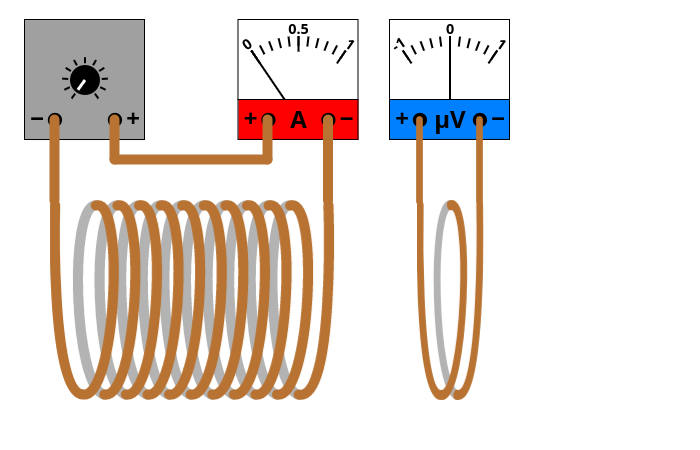
\includegraphics[width=0.95\textwidth]{induktions_andordnung}
            \caption{Induktionsandordnung \cite{leifi_induktions_anordnung}}
        \end{figure}
        \end{column}
    \end{columns}
\end{frame}

\subsection{Begriff der \textit{Induktivität}}
\begin{frame}
    \makeframetitle
    \begin{itemize}
        \item Formelzeichen: $L$
        \item Bezeichnet eine Eigenschaft eines Stromkreises bzw. Bauelements\\
            (besonders bei der \textit{Spule})
        \item Die Induktion beruht auf der Induktivität
        \item Unterscheidung zwischen \textit{Selbstinduktivität} und \textit{Gegeninduktivität}
    \end{itemize}
    \begin{block}{Information}
        Die \textit{Selbstinduktion} ist die \textit{Induktionswirkung} eines
        Stromes \textbf{auf seinen eigenen Leiterkreis}.
    \end{block}

\end{frame}

\begin{frame}
    \makeframetitle
    \begin{itemize}
        \item Die Selbstinduktivität $L$ ist abhängig von...
            \begin{enumerate}
                \item der Anzahl der Windungen $N$,
                \item der Länge $l$,
                \item der Fläche $A$,
                \item und der Permeabilität $\mu_r$ bzw. $\mu_0$
                    (\textbf{Naturkonstante})
            \end{enumerate}
          ...des Materials
          \item[\ding{212}] $L = \mu_0\mu_r \cdot \frac{AN^2}{l}$
    \end{itemize}
    \pause
    \begin{block}{Information}
         Die Permeabilität bezeichnet die Fähigkeit eines Materials durch ein äußeres Magnetfeld
         selbst magnetisiert zu werden.
    \end{block}
\end{frame}

\begin{frame}
    \makeframetitle
    \begin{figure}
        \begin{center}
            \includesvg[height=0.6\textheight]{./assets/current-carrying-coil.svg}
        \end{center}
        \caption{Größen der Induktivität an der Spule\cite{fuafev_image}}
    \end{figure}
\end{frame}

\begin{frame}
    \makeframetitle
    \begin{quote}
        Elektrische Verbraucher werden als \textbf{induktiv} bezeichnet, wenn
        sie ein \textbf{durchfließender}, \textbf{zeitlich
        \alert{veränderlicher} Strom} $I$ (z.B. beim Ein-/Ausschalten) über deren
        Klemmen eine zur Änderungsgeschwindigkeit $\frac{dI}{dt}$ proportionale
        Spannung $U_i$ hervorruft.
    \end{quote}
    \vspace{1cm}
    \pause
    \begin{block}{oder mit anderen Worten:}
        Der Betrag der Induktionsspannung $U_{i}(t)$ ist
        proportional zur Steigung der Funktion $I(t)$, also:
        \[
            U_i(t) = -L \cdot I'(t)
        \]
    \end{block}
\end{frame}

\begin{frame}
    \makeframetitle
    \begin{figure}
        \centering
        \begin{columns}
            \column{0.5\textwidth}
                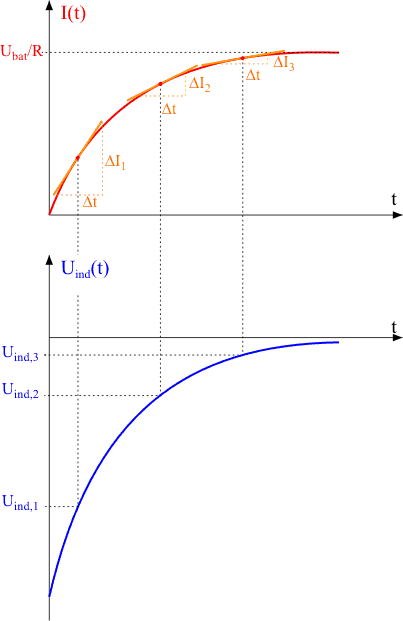
\includegraphics[height=0.80\textheight]{frame1.png}
            \column{0.5\textwidth}
                \caption{Darstellung des Zusammenhangs zwischen $U_{i}(t)$ und
                $I(t)$\cite{leifi_induktion_funktionen}}
        \end{columns}
    \end{figure}
\end{frame}

\begin{frame}
    \centering
    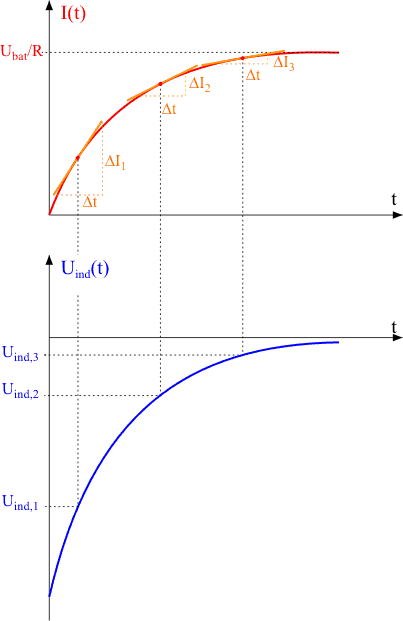
\includegraphics[height=0.90\textheight]{frame1.png}
\end{frame}

\subsection{Wirkung der \textit{Selbstinduktivität}}
\begin{frame}
    \makeframetitle
    \begin{itemize}
            \item $U_i$ \textit{wirkt} einer Spannung $U_0$
                \textit{entgegen} 
            \item $U_i$ ist \textit{gegengleich} der an der Spule $L$
                anliegenden Spannung $U_L$
    \end{itemize}
    \centering
    \begin{figure}
        \begin{circuitikz}[line width=1.0pt,scale=2.0]
            \draw
            (0, 2) to [battery1, a=$9\unit\V$, v=$U_0$] (0, 0)
            (0, 2) to [american inductor, l=$L$, v={$U_L$}] (2, 2)
            (2, 0) to [lamp] (2, 2)
            (2, 0) -- (0, 0)
            ;
            \draw
            (1, 1.5) node[]{$U_L = -U_i$} (2, 1.5)
            ;
        \end{circuitikz}
        \caption{Generischer Schaltkreis mit einer Spule $L$}
    \end{figure}
\end{frame}

\begin{frame}
    \makeframetitle
    \begin{columns}
        \column{0.5\textwidth}
        \begin{itemize}
            \item Der durch den Schaltkreis fließende
                Strom $I$ \textit{wächst allmählich} auf stationären Endwert
            \begin{itemize}
                \item[\ding{212}] \enquote{Hemmung} der Zunahme des Stromes
            \end{itemize}

            \item Gilt auch für einen \enquote{fallenden} Strom
        \end{itemize}
        \column{0.5\textwidth}
        \begin{figure}
            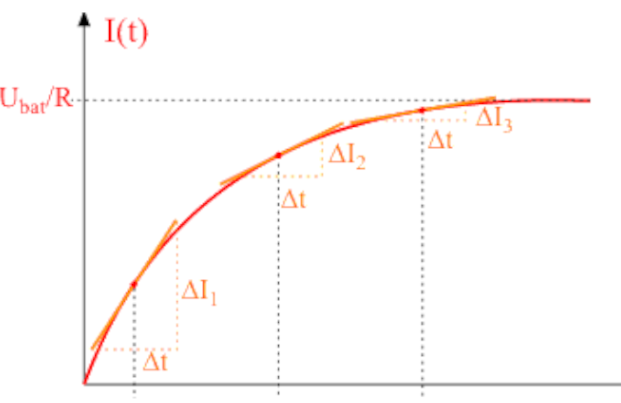
\includegraphics[width=0.95\textwidth]{IofT.png}
            \caption{$I(t)$\cite{leifi_induktion_funktionen}}
        \end{figure}
    \end{columns}
\end{frame}

\begin{frame}
    \makeframetitle
    \begin{figure}
        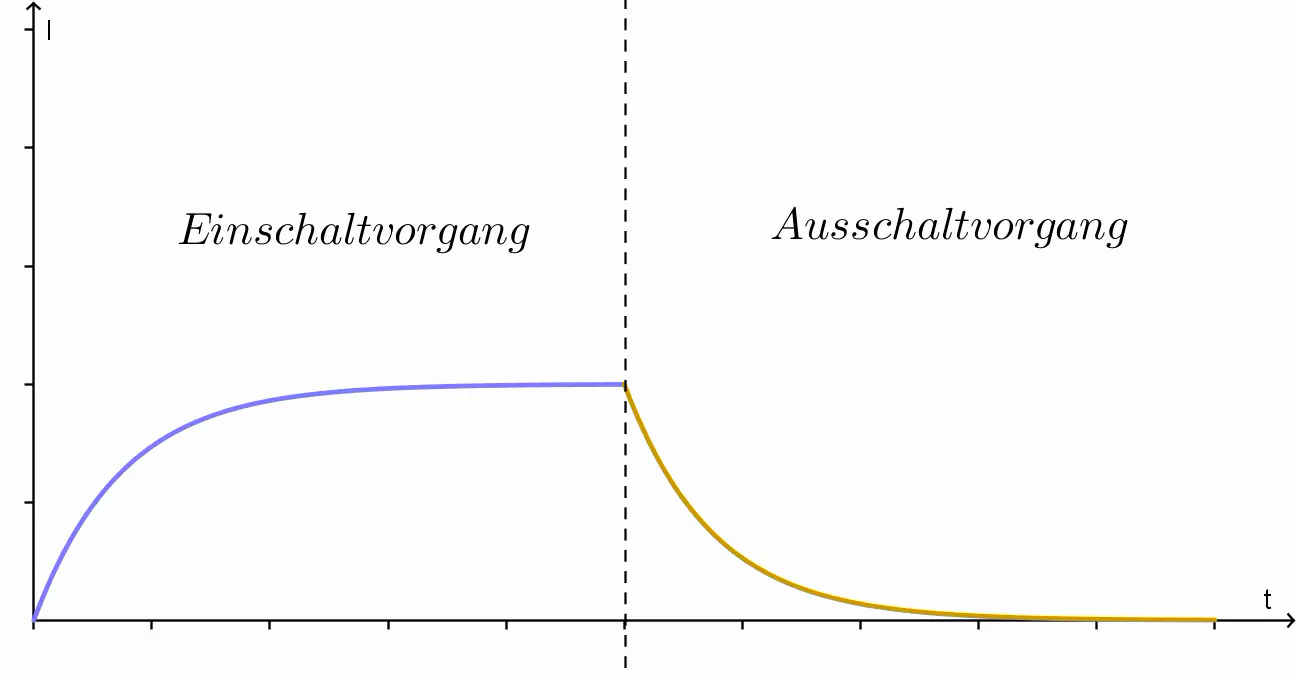
\includegraphics[height=0.6\textheight]{selbstinduktion_an_aus.png}
        \caption{Graph des Stromes während des Ein-/Ausschaltevorgangs\cite{abiweb_ein_aus}}
    \end{figure}
\end{frame}

\subsection{Formeln}
\begin{frame}
    \makeframetitle
    \begin{block}{Formelwerk}
        \begin{itemize}
            \item $U_i \sim -\frac{dI}{dt}$
            \item $U_i = -L \cdot \frac{dI}{dt}$
            \item $[L] = \frac{\left[|U_i|\right]}{\left[\frac{dI}{dt}\right]}
                = \frac{\unit\volt}{\frac{\unit\ampere}{\unit\second}}
                = \unit{\ohm\second} =: 1\unit{\henry}\text{(Henry)}$
        \end{itemize}
    \end{block}
\end{frame}
